\subsection{Сверточные нейронные сети}
\subsubsection{Обзор}
{\color{red} TODO Сверточные сети в контексте распознавания речи}


Сверточная нейронная сеть -- это алгоритм глубокого обучения, наиболее широко применяющийся для обработки визуальных данных, в рекомендательных системах\cite{cnn-recomendation-system} и при работе с естественным языком\cite{cnn-nlp}. Некоторые аспекты сверточных сетей были вдохновлены зрительной корой мозга животных\cite{cnn-neocognitron}. Предварительная обработка данных, требуемая в сверточных сетях, значительно ниже по сравнению с другими алгоритмами классификации.

Отличительными особенностями сверточных сетей являются их способность сохранять пространственную структуру входных данных и возможность автоматического обучения признакам/характеристикам, которые присущи конкретному классу объектов. Возможность запоминать и прослеживать пространственные связи во входных данных позволяют достигать высоких результатов в сферах компьютерного зрения и обработки естественного языка, недоступных для классических моделей с многослойным перцептроном и полностью связанных слоев.

\subsubsection{Архитектура}
\begin{figure}[h]
	\centering
	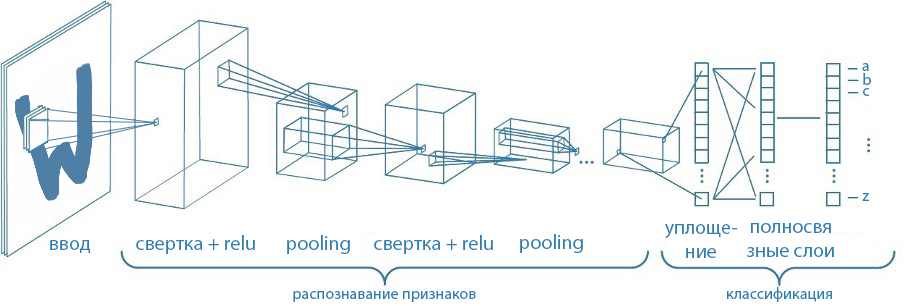
\includegraphics[width=1\textwidth]{cnn-architecture}
	\caption{Архитектура CNN сети.}
	\label{fig:cnn-architecture}
\end{figure}

Классическая сверточная сеть состоит из входного и выходного слоев, а также некоторого количества скрытых, внутренних слоев (Рис. \ref{fig:cnn-architecture}). Внутренние слои сверточной нейронной сети как правило состоят из серии слоёв, производящих \emph{свертку} с использованием ReLU\footnote{ReLU -- англ. Rectified Linear Unit, функция $f(x)=max(0,x)$} в качестве функции активации, после которой следуют остальные слои свертки, чередующиеся со слоями пулинга/субдискретизации. После прохождения нескольких слоев свертки и уплотнения, изображение из обычного набора пикселей с высоким разрешением превращается в более абстрактную карту признаков. В конце эти данные «уплощаются», то есть из тензора преобразуются в вектор и подаются на вход обычной полносвязной нейронной сети, которая тоже может состоять из нескольких слоев. В полносвязной части сети пространственная структура данных утрачивается, размерность в сравнении с исходным изображением значительно падает и основной задачей становится классификация на основе полученной карты признаков. Далее эти приемы будут рассмотрены подробнее.

\subsubsection{Слой свертки}
Отличительной чертой сверточных нейронных сетей является наличие слоев свертки, которые учитывают пространственную структуру изображения. Слои свертки направлены на извлечение ключевых признаков из изображения. На вход слоя свертки поступает тензор размерности (ширина изображения) $\times$ (высота изображения) $\times$ (глубина изображения), при обработке используется набор так называемых фильтров, за счет которых и производится свертка. Фильтр представляет собой тензор с тремя измерениями, где глубина совпадает с глубиной входного изображения, а размер фильтра выбирается как правило небольшой, например, 3$\times$3 или 5$\times$5.

Операция свертки заключается в следующем. Фильтр с определенным шагом передвигается по всевозможным позициям во входном изображении; на каждом шаге вычисляется сумма произведений соответствующих элементов фильтра с текущим рассматриваемым фрагментом входного изображения. Эта сумма записывается в выходной тензор, называемый картой признаков.
Таким образом, каждый сверточный нейрон обрабатывает только данные, попадающие в свое «поле зрения». Такой подход позволяет выполнять множество полезных операций: обнаружение краев, размытие или повышение резкости применением различных фильтров.
Шаг движения фильтра – один из гиперпараметров модели. Чаще всего он принимает значения 1 или 2.
Иногда применяется прием добавления отступов к изображению для того, чтобы размер исходного изображения совпадал с размером карты признаков.

\subsubsection{Pooling слой}
\emph{Pooling} слои уменьшают разрешение входного изображения, используя некоторую нелинейную операцию. Так, например, слой \emph{max-pooling} может уменьшить размер изображения вдвое, превращая фрагменты изображения размера 2$\times$2 в одно значение, выбирая максимальный из 4-х пикселей. Наиболее распространенными типами таких слоев являются:
\begin{itemize}
	\item max-pooling;
	\item pooling по среднему значению;
	\item pooling по сумме значений.
\end{itemize}

Типы слоев отличаются функцией, которая применяется к пикселям. Наиболее хорошо на практике показал себя метод \emph{max-pooling} \cite{cnn-max-pooling}. Действие слоя \emph{max-pooling} продемонстрировано на рисунке \ref{fig:max-pooling}.
\begin{figure}[h]
	\centering
	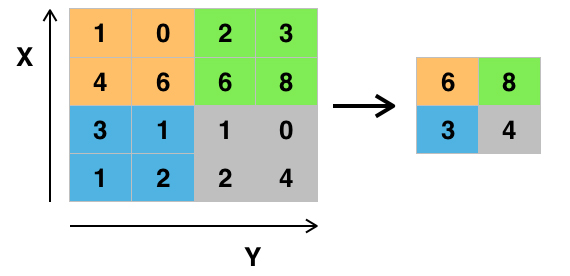
\includegraphics[width=0.7\textwidth]{max-pooling}
	\caption{Пример действия слоя \emph{max-pooling}.}
	\label{fig:max-pooling}
\end{figure}

\subsubsection{Слои ReLU}
\emph{ReLU} – функция, определяемая как $f(x)=max(0, x)$. Использование этой функции, по сравнению с другими, повышает нелинейность модели и качество принятия решений без внесения изменений в работу сверточных слоев\cite[с.~3]{cnn-imagenet}. Популярность \emph{ReLU} в качестве активационной функции обусловлена хорошей скоростью обучения моделей.

\subsubsection{Dropout слои}
Введение \emph{dropout}-слоев связано с проблемой переобучения сетей\cite{dnn-dropout}. Суть слоев этого типа в исключении случайных нейронов из рассмотрения при обучении. Это препятствует компонентам сети использовать взаимную адаптацию на данных для обучения, то есть предотвращает «заучивание» данных, на которых тренируется сеть.

\subsubsection{Полносвязные слои}
После части сети, отвечающей за извлечение признаков, идет несколько полносвязных слоев, которым подается уплощенная карта признаков для проведения классификации. На этом этапе сеть работает с признаками высокого уровня.